In this chapter, we will propose a few security notions for database encryption and study their properties. In particular, our security definitions aim to give the adversary the power to perform statistical attack on the database. We want to show that the intended security goals are indeed achievable by proving that some of the schemes we have constructed in the previous chapter are secure under these security definitions.

The goal of the adversary can be divided into two categories: 1) differentiate one database from the other, 2) identify plaintext-ciphertext pairs in the database. Both attacks will leak valuable information from the database and could potentially be abused by the adversary.

The key difference between PRIV adversary and adversaries considered in this chapter is that:
\begin{enumerate}
\item The adversary has access to the public key throughout the attack.
\item The adversary has access to the messages he challenged with throughout the attack.
\item The message space need not have high min-entropy.
\end{enumerate}
These assumptions give the adversary much more power but those things could indeed happen in practice. It is important to note that by giving the adversary the abilities above, he essentially has access to the decryption oracle too since the message space is usually polynomial in size.

In this section, we assume that the databases have same dimensions: they have the same number of columns and for each column, the number of possible attributes are the same. Further, the databases have the same number of real inputs. With regard to the security notion, the adversary is always given the encryption oracle to $PE$ (Recall that $PE$ is the probabilistic encryption scheme to generate the auxiliary column).




\section{Indistinguishability of distribution under chosen-plaintext attack (IND-DIST-CPA)}
The goal of the adversary in IND-DIST-CPA is to differentiate two databases with the same message space and different input distributions, with the power of encryption oracle to $DE$ and $PE$. Let the encryption scheme be $\Sigma = (Kg, \mathcal{E}, \mathcal{D})$. We define the IND-DIST-CPA adversary as $I = (I_d, I_m, I_g)$ where $I_d$ is the message set and input distribution generation algorithm that takes the security parameter $1^k$, the public keys to $DE$ and $PE$, and generates a message set $M$, two input distributions $\Gamma_0$ and $\Gamma_1$, and number of input messages $n$. $I_m$ is the message generation algorithm that takes in the security parameter $1^k$, public key $\pk$, and output of $I_d$, and generates two sequences of $n$ input messages $(m_0, m_1)$ sampled from $\Gamma_0$ and $\Gamma_1$ respectively. The challenger encrypts $m_b$ under the public key $\pk$ and returns the encrypted database $D$ to the adversary. Finally, $I_g$ is the guessing algorithm which takes input $1^k$, public key $\pk$, encrypted database $D$, output of $I_d$ and $I_m$, and returns $b'$ as the guess to the bit $b$.

We abuse the notation and write $Kg(1^k)$ to mean the key generation algorithm without specifying the input distribution, and $(\pk', \Gamma)$ to mean the public key associated to input distribution $\Gamma$. Then the adversary can be described as:
\begin{figure}[H]
	\begin{center}
		\procedure{$\text{Exp}_{\text{$\Sigma$, I}}^{\text{IND-DIST-CPA}}(1^k)$}{%
		\pcln b \sample \{0, 1\} \\
		\pcln (\pk', \sk) \gets Kg(1^k) \\
		\pcln (M, \Gamma_0, \Gamma_1, n) \gets I_d(1^k, \pk') \\
		\pcln (m_0, m_1) \gets I_m(1^k, \pk', M, \Gamma_0, \Gamma_1, n) \\
		\pcln D \gets \mathcal{E}(1^k, (\pk', \Gamma_b), m_b) \\
		\pcln b' \gets I_g(1^k, \pk', D, M, \Gamma_0, \Gamma_1, n, m_0, m_1) \\
		\pcln \pcreturn (b' = b)
		}
	\end{center}
	\caption{IND-DIST-CPA adversary}
\end{figure}

We require $I_m$ and $I_g$ to run in polynomial time in terms of the security parameter $1^k$. The advantage of an IND-DIST-CPA adversary is defined as
\begin{equation}
	\text{Adv}_{\text{$\Sigma$, I}}^{\text{IND-DIST-CPA}}(1^k) = \prob{\text{Exp}_{\text{$\Sigma$, I}}^{\text{IND-DIST-CPA}}(1^k) \Rightarrow \text{true}} - \prob{\text{Exp}_{\text{$\Sigma$, I}}^{\text{IND-DIST-CPA}}(1^k) \Rightarrow \text{false}}.
\end{equation}

With a standard probability argument, we can show that
\begin{equation}
\text{Adv}_{\text{$\Sigma$, I}}^{\text{IND-DIST-CPA}}(1^k) = 2\prob{\text{Exp}_{\text{$\Sigma$, I}}^{\text{IND-DIST-CPA}}(1^k) \Rightarrow \text{true}} - 1.
\end{equation}

We say that scheme $\Sigma$ is secure under IND-DIST-CPA if $\text{Adv}_{\text{$\Sigma$, I}}^{\text{IND-DIST-CPA}}(1^k)$ is negligible in $k$.


\begin{theorem} \label{thm IND-DIST-CPA 1}
Suppose $I$ is an IND-DIST-CPA adversary against \texttt{Padding1}. Then there exists an IND-CPA adversary $A$ against $PE$ such that
\begin{equation}
	\text{Adv}_{\texttt{Padding1}, \text{I}}^{\text{IND-DIST-CPA}} \leq \text{Adv}_{\text{$PE$, A}}^{\text{IND-CPA}} \label{c4 tm1}
\end{equation}
\end{theorem}

\textit{Proof:} Suppose that we have a distinguisher $B$ for databases constructed with \texttt{Padding1}. We wish to construct an IND-CPA adversary $A$ against $PE$. Because we have access to the encryption oracles of $DE$ and $PE$, the adversary can construct databases specified in \texttt{Padding1} on his own.

We start by picking message set $M$ and input distributions $\Gamma_0$ and $\Gamma_1$. We can simply set $M = \{1, \cdots, k\}$ for some large $k$, and $\Gamma_0(i) = \Gamma_1(i)$ for all $i \geq 3$. We also require $\Gamma_0(1) = \Gamma_1(2)$ and $\Gamma_0(2) = \Gamma_1(1)$, where $\Gamma_0(1) = 2 \Gamma_0(2)$ and $\Gamma_0(1) > 0$. In short, we make input distribution on all attributes equal except the first two. For the first two attributes, they are swapped for the two databases. We generate inputs to be encrypted according to the two distributions and name them $m_0$ and $m_1$ respectively.

For adversary A, we set the message generation algorithm to be a deterministic algorithm that outputs $(True, False)$. The challenger encrypts one of them and outputs $c$. To guess the underlying plaintext of $c$, we define a new encryption scheme that is similar to \texttt{Padding1}:
\begin{figure}[H]
	\begin{center}
		\procedure{$Enc(m_0, c)$}{%
			\pcln D \gets () \\
			\pcln  (x_1, \cdots, x_n) \gets m_0 \\
		  	\pcln \pcfor i = 1 \cdots n \\
		  	\pcln \t \pcif x_i = C_1 \\
		  	\pcln \t \t D \gets \$(D, (\overbar{Enc_1}(x_i) \ ||\ c)) \\
		  	\pcln \t \pcelse D \gets \$(D, (\overbar{Enc_1}(x_i) \ ||\ \overbar{enc_2}(True))) \\
		  	\pcln \t \pcfor x \in C \backslash \{x_i\} \\
		  	\pcln \t \t D \gets \$(D, (\overbar{Enc_1}(x) \ ||\ \overbar{Enc_2}(False)))
		}
	\end{center}
	\caption{Modified encryption scheme from \texttt{Padding1}}
\end{figure}
where $C$ is the set of attributes and $C_1$ denotes the first attribute. The only difference in this scheme from the original one is that if the encrypted attribute is the first one, $c$ is used then a fresh encryption of $True$. If $c$ is indeed an encryption of $True$, then the distinguisher $B$ is able to identify the database encrypted this way as one that comes from $\Gamma_0$.

But all these happens with probability bounded by the advantage of IND-DIST-CPA adversary. Thus the desired inequality. $\square$




\begin{theorem}
	Suppose $I$ is an IND-DIST-CPA adversary against \texttt{Padding3}. Then there exists an IND-CPA adversary $A$ against $PE$ such that
	\begin{equation}
	\text{Adv}_{\texttt{Paddign3}, \text{I}}^{\text{IND-DIST-CPA}} \leq \text{Adv}_{\text{$PE$, A}}^{\text{IND-CPA}}
	\end{equation}
\end{theorem}

\textit{Proof:} Let $\xi_1, \cdots, \xi_k$ be the counts of the attributes in the encrypted database. Recall in theorem \ref{thm frequency dist} we have shown that $\xi_i$'s have the same distribution. Given that the input distribution is $\Gamma$, we must have
\begin{equation*}
	\prob{(\xi_1, \cdots, \xi_k) \mid \Gamma} = \prob{(\xi_1, \cdots, \xi_k)},
\end{equation*}
that is, the joint distribution of the counts is independent of the input distribution. Therefore, we conclude that
\begin{equation*}
	\prob{(\xi_1, \cdots, \xi_k) \mid \Gamma_0} = \prob{(\xi_1, \cdots, \xi_k) \mid \Gamma_1},
\end{equation*}
for any input distributions $\Gamma_0$ and $\Gamma_1$. In particular, the adversary has no advantage to tell if the encrypted database comes from the first distribution or the second. Therefore, the problem is reduced to theorem \ref{thm IND-DIST-CPA 1}, hence the advantage stated above. $\square$




\section{Indistinguishability of Ciphertext under Statistical Attack (IND-STAT)}
In this section, we consider a somewhat weak adversary who has no access to the encryption oracle to $DE$. His goal is to identify at least a pair of plaintext-ciphertext, given that he knows the set of plaintexts and their frequencies in the database. In fact, in the security model, we give him much more power - he has the freedom to choose what database he wants to encrypt, and in which order the plaintexts should appear.


Let the encryption scheme be $\Sigma = (Kg, \mathcal{E}, \mathcal{D})$. We define the IND-STAT adversary as $I = (I_m, I_g)$ where $I_m$ is the message generation algorithm that takes in the security parameter $1^k$, public key $\pk$ and generates a sequence of messages $M = \{m_1, \cdots, m_n\}$. $I_g$ is the guessing algorithm which takes input security parameter $1^k$, public key $\pk$, encrypted database $D$ and messages $M$, and returns a pair of message and ciphertext $(m, c)$. He wins if he can identify a valid pair with probability significantly higher than $\frac{1}{k}$, where $k$ is the number of attributes in the database.
\begin{figure}[H]
	\begin{center}
		\procedure{$\text{Exp}_{\text{$\Sigma$, I}}^{\text{IND-STAT}}(1^k)$}{%
			\pcln (\pk, \sk) \gets Kg(1^k) \\
			\pcln M = \{m_b^1, \cdots, m_b^n\} \gets I_m(1^k, \pk) \\
			\pcln D \gets \mathcal{E}(1^k, \pk, \{m_b^1, \cdots, m_b^n\}) \\
			\pcln (m, c) \gets I_g(1^k, \pk, D, M) \\
			\pcln \pcreturn (m, c)
		}
	\end{center}
	\caption{IND-STAT adversary}
\end{figure}

We require $I_m$ and $I_g$ to run in polynomial time in terms of the security parameter $1^k$. The advantage of an IND-STAT adversary is defined as
\begin{align*}
\text{Adv}_{\text{$\Sigma$, I}}^{\text{IND-STAT}}(1^k) = 
\prob{(m,c) \Leftarrow \text{Exp}_{\text{$\Sigma$, I}}^{\text{IND-STAT}}(1^k), Enc(m) = c}  - \frac{1}{k}. \numberthis
\end{align*}


It is important to note that the adversary does \textbf{not} have access to the encryption oracle for $DE$. Schemes that cannot achieve IND-STAT security are advised to not be used in practice. In particular, we have seen that trivial deterministic encryption on statistical databases is vulnerable to frequency analysis \cite{Naveed:2015:IAP:2810103.2813651}. Our adversary is compatible with that attack. The auxiliary data used in the attack can be viewed as the input messages in our security model.

There are a few key results we wish to highlight in this section. First of all, we claim that IND-STAT is incomparable with IND-DIST-CPA. Furthermore, we will show that IND-STAT is not achievable if the adversary is given the encryption oracle to $DE$. Thus, none of the schemes we have proposed in the previous chapter can achieve any security in practice. Finally, we want to argue that \texttt{Padding1} and \texttt{Padding3} can be modified such that we can assume that the adversary does not have access to the encryption oracle to $DE$, thus concluding that those schemes are secure in practice.




\subsection{IND-DIST-CPA and IND-STAT are not Comparable} \label{thm5}
Intuitively speaking, IND-DIST-CPA captures the security goal where given two databases of equal size, one should not be able to distinguish them. However, it does not mean that the two databases themselves are invulnerable to statistical attacks in the first place.

\begin{theorem}
	IND-DIST-CPA security does not imply IND-STAT security.
\end{theorem}

\textit{Proof:} \\
To prove the statement, we wish to construct a scheme that is IND-DIST-CPA secure but not IND-STAT secure. 

\textbf{Part 1: \texttt{Padding2}$^{+}$ is IND-DIST-CPA secure} \\
\texttt{Padding2} in general is not IND-DIST-CPA secure. This is because the counts on the attributes converges to different distributions. However, if we restrict the scheme to a subset of input distributions that are close to each other, it is possible to achieve IND-DIST-CPA security. Formally, we define \texttt{Padding2$^+$} to be the same as \texttt{Padding2}, except that the message distribution is constrained the following way. Let $\Pi$ be some distribution on the message space, we require all message distributions $\Pi_0$ challenged by the adversary to be such that $\Pi(j) = \Pi_0(j) \ \forall j \geq 3$, and $\abs{\Pi_0(j) - \Pi_i(j)} \leq \delta$ for some $\delta << 1$. To distinguish the two databases, with $n$ insertions, the advantage of the adversary $I$ is
\begin{equation}
	\text{Adv}_{\text{$\Sigma$, I}}^{\text{IND-DIST-CPA}}(D) \leq \text{Adv}_{\text{$PE$, A}}^{\text{IND-CPA}} + \abs{\prob{0 \leftarrow B_{\text{stat}}(D)} - \prob{1 \leftarrow B_{\text{stat}}(D)}}
\end{equation}
where the second part of the advantage is generated by some statistical adversary $B_\text{stat}$. We argue that by making the restriction above, we can generate two input distributions such that the statistical advantage is insignificant. See appendix \ref{Justification of claim P2 1} for a justification. Since the statistical distance between the two databases are bounded, no statistical adversary can do better than that. We conclude that \texttt{Padding2$^+$} is IND-DIST-CPA secure.


\textbf{Part 2: \texttt{Padding2}$^{+}$ is not IND-STAT secure} \\
It is left to show that \texttt{Padding2}$^{+}$ does not meet the security definition of IND-STAT. We hereby propose an attack against \texttt{Padding2}$^{+}$. The attack relies on the stochastic nature of the encryption algorithm - since the variance of the attributes are different, the likelihoods to observe a given count on the attributes are different.

Without loss of generality, assume that we want to differentiate attributes 1 and 2 given the encrypted database. Recall that in theorem \ref{thm frequency dist}, we have proven that the variance of the counts of the attributes is equal to $s_{n(p+1)}^2(j) = n \cdot s^2(j)$, where $s^2(j) = \sum_{i= 0}^{p} \Pi_i(j) (1 - \Pi_i(j))$. Assume that $s^2(1) > s^2(2)$, then the distribution of the counts can be plotted as:

\begin{figure}[H]
	\centering
	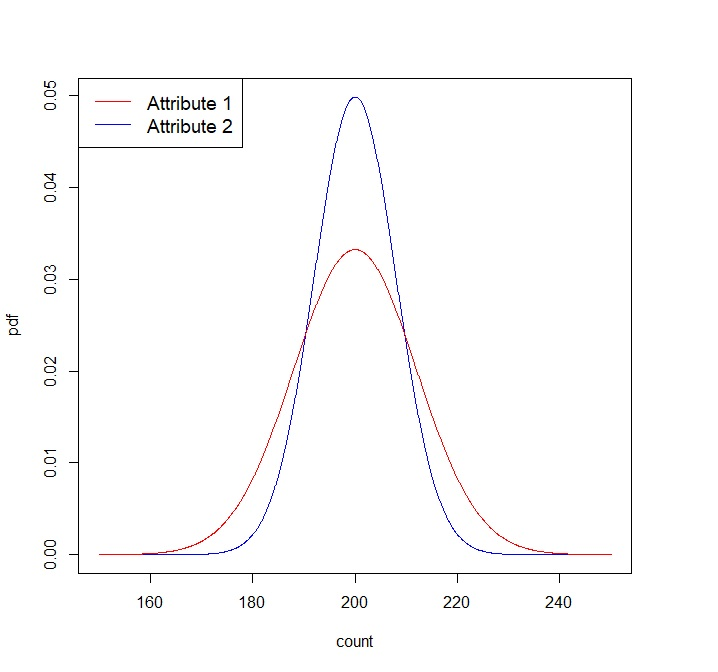
\includegraphics[scale=0.5]{./Images/Distributions.jpg}
	\caption{Distribution of the count of the two attributes} \label{distribution plot}
\end{figure}

In the figure, the mean of the count of the two attributes is 200, and the variances are 64 and 144 respectively. As it can be seen, the height of the probability density function (pdf) for attribute 1 is much lower than that of attribute 2. This means that the count of attribute 1 is less likely to be close to the mean (200 in this case) than attribute 2. Suppose that we see that, in the encrypted database, some encrypted attribute occurs 200 times, our guess would be that this encryption corresponds to attribute 2 in this example. Now we will formalize this attack.

We start by defining statistical distance between two distributions.
\begin{definition}[Statistical distance] \label{statistical distance}
	Let $D_1$ and $D_2$ be two distributions, with pdf $p_1(\cdot)$ and $p_2(\cdot)$ respectively. Statistical distance $d(\cdot,\cdot)$ between $D_1$ and $D_2$ is defined to be:
	\begin{equation}
		d(D_1, D_2) := \int_{-\infty}^{\infty} \lvert p_1(x) - p_2(x) \rvert \  dx.
	\end{equation}
\end{definition}

It is not hard to prove that this definition of statistical distance is a metric. Graphically, this corresponds to the area between the pdf's of the two distributions. It can also be think of as the advantage we have to distinguish two distributions: consider the case where $D_1 = D_2$, then by definition, $d(D_1, D_2) = 0$ so it is impossible for us to differentiate $D_1$ from $D_2$; if $D_1$ and $D_2$ have non-intersecting supports, then $d(D_1, D_2) = 2$, and we can differentiate $D_1$ from $D_2$ with certainty.

In this case, we are interested in two normal distributions with same mean and different variance. We want to derive a lower bound on $d(D_1, D_2)$ given that $D_1 \sim \mathcal{N}(\mu, \sigma^2)$, and $D_2 \sim \mathcal{N}(\mu, \gamma^2\sigma^2)$.

\begin{theorem} \label{thm lb on statistical distance}
	Let $D_1 \sim \mathcal{N}(\mu, \sigma^2)$, and $D_2 \sim \mathcal{N}(\mu, \gamma^2\sigma^2)$ for some $\gamma > 1$. Then
	\begin{equation}
		d(D_1, D_2) \geq 2 \cdot \left( \Phi\left( \gamma\left( \frac{2}{\gamma^2 - 1} \log(\gamma) \right)^{0.5} \right) - \Phi\left( \left( \frac{2}{\gamma^2 - 1} \log(\gamma) \right)^{0.5} \right) \right),
	\end{equation}
	where $\Phi(\cdot)$ is the cdf for standard normal distribution.
\end{theorem}

\textit{Proof:} See appendix \ref{Proof of lb on statistical distance}.

The idea is that, by making $\gamma$ large, we can make $d(D_1,D_2)$ arbitrarily large, so that the advantage generated by the statistical distance is not negligible.

We are ready to present our attack based on \texttt{Padding2}$^{+}$. The idea is to generate the database such that variance of all attributes are equal except one of them - which we want it to be $\gamma^2$ times smaller. Then the encrypted attribute in the database differs the least from the expectation is more likely to be the variable with the smallest variance. But before doing that, we need to show that it is possible to achieve the variances claimed above.

Proof of the claim: Following the standard notation we use in this report, let there be $k$ attributes and $p$ additional insertions, both to be determined later. The idea is to set the distribution of plaintext to $\Pi_0(1) = 1 - k\delta$, and all other $\Pi_0(j)$'s for some $\delta << 1$. We can see immediately if we do so, then $p = k - 1$, if $\delta$ is sufficiently small. Then the variances are:
\begin{align*}
	s^2(1) = & (1 - k\delta) \cdot k \delta + p \cdot \delta (1 - \delta) \\
		   = & (k+p) \delta - (k^2 + p) \delta^2 \\
		   = & (2k - 1) \delta - (k^2 + k - 1) \delta^2 \\
    s^2(j) = & \delta (1 - \delta) + p \frac{1 - \delta}{p} \cdot \left( 1 - \frac{1 - \delta}{p} \right) \\
    	   = & \left(1 - \frac{1}{p}\right) - \left( 1 - \frac{2}{p} \right) \delta - \mathcal{O}(\delta^2) \\
    	   = & \left(1 - \frac{1}{k-1}\right) - \left( 1 - \frac{2}{k-1} \right) \delta - \mathcal{O}(\delta^2) \ \text{for all } j \neq 1
\end{align*}

So the ratio of $s^2(j)$ to $s^2(1)$ for large $k$ is approximately
\begin{align*}
	\frac{1 - \delta}{(2k - 1) \delta - (k^2 + k - 1) \delta^2} 
\end{align*}
which can obviously be made arbitrarily large by picking a large $k$ and $\delta = \mathcal{O}(k^{-2})$. $\square$

\textbf{Attack on Variance} Define he adversary to IND-STAT on \texttt{Padding2}$^{+}$ to be $I = (I_m, I_g)$. Where $I_m$ fixes a $\gamma$ that is large enough, generates plaintext distribution by the process described above with that $\gamma$, and generate $n >> k$ messages sampled from the plaintext distribution. Upon receiving the encrypted database, $I_g$ picks the encrypted attribute $c$ which has its count closest to the mean, and returns his guess as $(m_0,c)$, where $m_0$ is the first attribute with $\Pi_0(1) = 1 - k\delta$.

We can compute the success rate of the attack directly. Let $\xi_1, \cdots, \xi_k$ be random variables corresponds to the counts on the attributes in the encrypted database. So by theorem \ref{thm frequency dist}, we have $\xi_i \sim \mathcal{N}(\frac{n \cdot (p+1)}{k}, n \cdot s^2(i))$. Let $\mu = \frac{n \cdot (p+1)}{k}$, then the probability that attribute 1 is the closest one to the mean can be expressed as:
\begin{align}
  & \prob{\text{attribute 1 is the closest one to the mean}} \\
= & \int_{x} \prob{\text{attribute takes value } x} \cdot \prob{\text{all other attributes takes value further than } x \text{ from } \mu} \ dx \label{VA 1} \\
\approx & \int_{-\infty}^{\infty} p(\xi_1 = x) \cdot \prod_{i = 2}^{k} p(\abs{\xi_i - \mu} > \abs{x - \mu}) \ dx \label{VA 2}\\
= & \int_{-\infty}^{\infty} p(\xi_1 = x) \cdot \prod_{i = 2}^{k} p(\xi_i > \mu + \abs{x - \mu} \text{ or } \xi_i < \mu - \abs{x - \mu}) \ dx \label{VA 3} \\
= & \int_{-\infty}^{\infty} \phi\left(\frac{x - \mu}{\sqrt{n} \cdot s(1)}\right) \cdot \prod_{i = 2}^{k} 2 \cdot \Phi\left(\frac{- \abs{x - \mu}}{\sqrt{n} \cdot s(i)}\right) \label{VA 4}
\end{align}

Equation \ref{VA 1} is just a re-statement of the event. In equation \ref{VA 2}, we have converted the description of the events into their mathematical forms. In the process, we have ignored the contribution of covariance to the likelihood. To go from equation \ref{VA 2} to equation \ref{VA 3}, we turn the event $\abs{\xi_i - \mu} > \abs{x - \mu}$ into expressions with $\xi_i$ on one side and other things on the other, to make it computable. Finally, equation \ref{VA 4} is a direct computation from equation \ref{VA 3}, where $\phi(\cdot)$ and $\Phi(\cdot)$ are the probability density function (pdf) and cumulative density functions respectively.

Unfortunately, it is only possible to compute the integral analytically if $k = 2$. But our goal is to show the existence and correctness of the attack, it is sufficient to use numerical integration to compute this.

\textbf{Numerical Example} As a numerical example, we consider the following input distribution with $k = 6$ and $p = 5$:
\begin{align*}
	\Pi_0(j) = & \begin{cases*}
				   0.95 \quad \text{if } j = 1 \\
				   0.01 \quad \text{otherwise}
		  	     \end{cases*}, \\
	\Pi_i(j) = & \begin{cases*}
				   0.01 \quad \text{if } j = 1 \\
				   0.198 \quad \text{otherwise}
				 \end{cases*} \quad \text{for } i = 1, \cdots,5. 
\end{align*}
The integral in equation \ref{VA 4} in this case evaluates to $0.4054$, which means there is $40.54\%$ chance for the count of attribute 1 in the encrypted database to be the closest one to the mean. This gives an advantage of $0.4054 - \frac{1}{6} = 23.9\%$, which is clearly not negligible. We verify the result by simulating the attack. An advantage of $24.0\%$ is found, with $n = 8000$, and $50,000$ simulation runs of the encryption scheme. $\square$




\textbf{Discussion of the Attack} Note that in equation \ref{VA 4}, the advantage depends on $n$, the number of plaintexts in the database. But our numerical experiments suggest that this dependency is irrelevant. This can be explained intuitively by thinking of the advantage as something generated by the ratio of the variances. In that case, the number of insertions is not a factor.

We argue that the advantage increases as $\gamma$, the ratio between the variances increases. This is verified with a series of experiments similar to the one showed above. The results are summarised in figure \ref{VA advantage table}.

There is also a nice interpretation of the result in terms of statistical distance we have defined in definition \ref{statistical distance}. We expect to differentiate two distributions more easily if they have larger statistical distance. This is indeed the case. Using the estimated statistical distance in theorem \ref{thm lb on statistical distance}, we find a strong correlation between statistical distance and theoretical advantage, as shown in figure \ref{VA advantage table}.

\begin{figure}[H]
	\centering
	\begin{tabular}{cccc}
		$\gamma$ & Advantage (Theoretical est.) & Advantage (Simulation) & Statistical distance \\ \hline
		2.879    & 23.9\%	 & 24.0\% 	& 0.469 \\
		2.073	 & 15.0\%	 & 15.1\%	& 0.338 \\
		1.723    & 10.5\%    & 10.4\%	& 0.257 \\
		1.386    & 5.83\%    & 5.91\%	& 0.157 \\
		1.087    & 1.36\%    & 1.23\%	& 0.040  \\
		1.000    & 0.00\%    & -		& 0.000
	\end{tabular}
	\caption{Relation between $\gamma$ and advantage of Variance attack}
	\label{VA advantage table}
\end{figure}




There are also schemes that are IND-STAT secure but not IND-DIST-CPA secure.
\begin{theorem}
	IND-STAT security does not imply IND-DIST-CPA security.
\end{theorem}

\textit{Proof:} We give an encryption scheme that is IND-STAT secure but not IND-DIST-CPA secure. The construction is similar to \texttt{Padding1}. In addition to the database generated by \texttt{Padding1}, we pad the database further with a dummy attribute, generated by XOR of first two plaintexts in the database. More formally, we define the encryption scheme \texttt{Padding4} = $(Kg, Enc, Dec)$ as:

\begin{figure}[H]
	\begin{center}
		\begin{pchstack}
			\procedure[linenumbering]{$Enc(m_1, \cdots, c_n)$}{%
				\pcfor i \in 1 \cdots n	\\
				\t	D \gets \$(D, \texttt{Padding1.}Enc(m_i)) \\
				\t  D \gets \$(D, Enc_1(m_1 \oplus m_2), Enc_2(False)) \\
				\pcreturn D
			}
		\end{pchstack}
	\end{center}
	\caption{Encryption scheme for \texttt{Padding1}}
\end{figure}
where $\texttt{Padding1.}Enc(\cdot)$ is the encryption function defined for \texttt{Padding1}. And $Kg$ and $Dec$ are the key generation function and decryption functions of \texttt{Padding1} respectively.

\textbf{Part 1: \texttt{Padding4} is IND-STAT secure} \\
We want to show that it is impossible for a statistical attack on the encrypted database generated by \texttt{Padding4}. We rely on the fact that if the attribute columns of the encrypted database is independent of underlying plaintexts, then no statistical information can be inferred. Indeed, the attributes in the encrypted database are in the same order, and have the same number of occurrences regardless of the input plaintexts. Thus, \texttt{Padding4} is IND-STAT secure.

\textbf{Part 2: \texttt{Padding4} is not IND-DIST-CPA secure}
On the other hand, it is easy to attack the database in the IND-DIST-CPA setting. The adversary can generate two raw databases $\{m_1,m_2, \cdots, m_n\}$ and $\{m_1', m_2', \cdots, m_n'\}$ such that $m_1 \oplus m_2 \neq m_1' \oplus m_2'$. After the challenger returns one of the encrypted database, the adversary uses the encryption oracle of $DE$ to encrypt $m_1 \oplus m_2$ and $m_1' \oplus m_2'$. He returns his guess bit $b$ as 0 if the encrypted database contains the encryption of $m_1 \oplus m_2$ and 1 otherwise. The advantage of the adversary is 1. $\square$




\subsection{Security Proofs}
In this section, we will prove that \texttt{Padding1} and \texttt{Padding3} are IND-STAT secure. Security proof for \texttt{Padding1} is almost identical to that of \texttt{Padding4} so we will leave it to the readers. For \texttt{Padding3}, we will use an information-theoretic argument to prove its security.

\begin{theorem}
	\texttt{Padding3} is IND-STAT secure.
\end{theorem}

\textit{Proof:} Recall in theorem \ref{thm frequency dist} we have shown that the distribution of the counts converges to $\mathcal{N}(\frac{n \cdot (p+1)}{k}, n \cdot s^2(j))$ for large $n$. But by construction of \texttt{Padding3}, $s^2(i) = s^2(j) \ \forall i,j$, so we can write the distribution as $\mathcal{N}(\frac{n \cdot (p+1)}{k}, n \cdot s^2)$ for some common variance $s^2$. The covariances between the attributes are equal by construction too. In this form, all parameters of the distribution are available in the public key so the adversary cannot infer anything unknown from the statistics of the database. Therefore, it is impossible to use statistical methods to identify plaintext-ciphertext pairs. $\square$

\textbf{Discussion} The proof above would not work for the trivial encryption scheme. This is because the counts of the encrypted attributes can be modelled by deterministic variables $\xi_1, \cdots, \xi_n$, and these do depend on the count of the input attributes. So by learning these variables, one reveals information about the underlying plaintext.




\subsection{On the Assumption of Absence of Encryption Oracle of $DE$}
Curious readers would realise by this point that IND-STAT is only achievable if the adversary has no access to the encryption oracle of $DE$ - otherwise, he can simply query the encryption oracle with one of the messages he challenged with and return that message with the answer to the query as his output of the game. He wins the game with certainty. But it is not reasonable to make this assumption, given that the underlying encryption scheme is a public-key one. Thus, we have to use something different.

Recall that our database encryption scheme is intended to protect the users from malicious third-party service providers. Since it suffices for the encryption to be deterministic to achieve efficient database queries, we may not want to give the service provider a way to decipher the entries of the database. This can be done easily by making the key `symmetric', i.e. only the users have access to the key and the insertions to the database are done after encryption locally by the users. The same argument can be applied to $PE$ part of the encryption scheme.




\section{Indistinguishability of distribution (IND-DIST)}
In the absence of encryption oracle to $DE$, IND-DIST-CPA is no longer a valid security notion for our application. To adapt to the changes, we define indistinguishability of distribution (IND-DIST) to be the new security notion which is identical to IND-DIST-CPA except that:
\begin{enumerate}
\item The adversary no longer has access to the encryption oracle to $DE$ and $PE$,
\item He can challenge with two completely different message spaces, as long as $p$ and $k$ are fixed.
\end{enumerate}

Let the encryption scheme be $\Sigma = (Kg, \mathcal{E}, \mathcal{D})$. Formally, we define the adversary against $\Sigma$ as tuple $I = (I_d, I_m, I_g)$. $I_d$ takes in the security parameter $1^k$ and generates plaintext sets $M_0, M_1$ and corresponding input distributions (only the actual plaintexts) $\Gamma_0, \Gamma_1$, and the number of inputs $n$. We write the output as $((M_0, \Gamma_0), (M_1, \Gamma_1), n)$. $I_m$ is the message generation algorithm which takes security parameter $1^k$, output of $I_d$, and generate two sequences of inputs to the database $(m_0, m_1)$ (only the actual plaintexts) according to $\Gamma$. The challenger encrypts the inputs $m_b$ using his public key and returns the encrypted database $D$ to the adversary. Finally, $I_g$ is the algorithm which takes input security parameter $1^k$, output of $I_d$ and $I_m$ and encrypted database $D$, and output his guess bit $b'$. He wins if $b = b'$.


\begin{figure}[H]
	\begin{center}
		\procedure{$\text{Exp}_{\text{$\Sigma$, I}}^{\text{IND-DIST}}(1^k)$}{% 
			\pcln b \sample \{0, 1\} \\
			\pcln ((M_0, \Gamma_0), (M_1, \Gamma_1), n) \gets I_d(1^k) \\
			\pcln (\pk, \sk) \gets Kg(1^k, M_b, \Gamma_b) \\
			\pcln (m_0, m_1) \gets I_m(1^k, (M_0, \Gamma_0), (M_1, \Gamma_1), n) \\
			\pcln D \gets \mathcal{E}(1^k, m_b, \pk) \\
			\pcln b' \gets I_g(1^k, (M_0, \Gamma_0), (M_1, \Gamma_1), n, (m_0, m_1), D) \\
			\pcln \pcreturn (b' = b)
		}
	\end{center}
	\caption{IND-DIST adversary}
\end{figure}


The adversary $I$ is legit if:
\begin{enumerate}
\item $n$ is large enough for CLT to hold (we recommend $n \geq 100$),
\item $\abs{M_0} = \abs{M_1}$,
\item Inputs $m$ are truly sampled according to $\Gamma$.
\item All three algorithms runs in polynomial time.
\end{enumerate}
Note that in this setting, the adversary is allowed to generate input distributions $\Gamma_0$ and $\Gamma_1$ such that they are equal.

The advantage of an IND-DIST adversary is defined as
\begin{equation}
\text{Adv}_{\text{$\Sigma$, I}}^{\text{IND-DIST}}(1^k) = \prob{\text{Exp}_{\text{$\Sigma$, I}}^{\text{IND-DIST}}(1^k) \Rightarrow \text{true}} - \prob{\text{Exp}_{\text{$\Sigma$, I}}^{\text{IND-DIST}}(1^k) \Rightarrow \text{false}}.
\end{equation}

With a standard probability argument, we can show that
\begin{equation}
\text{Adv}_{\text{$\Sigma$, I}}^{\text{IND-DIST}}(1^k) = 2\prob{\text{Exp}_{\text{$\Sigma$, I}}^{\text{IND-DIST}}(1^k) \Rightarrow \text{true}} - 1.
\end{equation}

We say that scheme $\Sigma$ is secure under IND-DIST if $\text{Adv}_{\Sigma, \text{I}}^{\text{IND-DIST}}(1^k)$ is negligible in $k$.


\textbf{A Useful Fact:} Define the maximum key probability $\text{mkp}_\Sigma(1^k)$ for encryption scheme $\Sigma = (Kg, \mathcal{E}, \mathcal{D})$ with security parameter $1^k$ as:
\begin{equation}
	\text{mkp}_\Sigma(1^k) = \max_{v} \prob{\pk = v \mid (\pk, \sk) \gets Kg(1^k)} + \max_{w} \prob{\sk = w \mid (\pk, \sk) \gets Kg(1^k)}
\end{equation}

We claim that if $\Sigma$ is IND-CPA secure, then $\text{mkp}_\Sigma(1^k)$ is negligible in $k$. 

\textit{Proof:} The proof can be seen as a generalization to proposition 4.1 in \cite{Bellare2007}. We suppose for the sake of contrary that $\text{mkp}_\Sigma(1^k)$ is not negligible, and we demonstrate that we can construct an IND-CPA adversary against $\Sigma$. By construction, if $\text{mkp}_\Sigma(1^k)$ is not negligible then either $\max_{v} \prob{\pk = v \mid (\pk, \sk) \gets Kg(1^k)}$ is not negligible or $\max_{w} \prob{\sk = w \mid (\pk, \sk) \gets Kg(1^k)}$ is not.

In the first case, it means that certain public key is generated with significant probability. We can simply run the key generation algorithm repetitively until the public key part of the key is that key. If $\max_{v} \prob{\pk = v \mid (\pk, \sk) \gets Kg(1^k)} = p$, then we only need $\mathcal{O}(1/p)$ runs of the key generation algorithm to find out the key pair. After that, we can freely decrypt any message we want, so we break $\Sigma$ with certainty.

Similarly, if $\max_{w} \prob{\sk = w \mid (\pk, \sk) \gets Kg(1^k)} = p$ is not negligible, we can run the key generation algorithm $\mathcal{O}(1/p)$ times to find the corresponding secret key, and decrypt any message we want afterwards. $\square$


\begin{theorem} \label{thm IND-STAT 1}
Let $I = (I_d, I_m, I_g)$ be the IND-STAT adversary against \texttt{Padding1}, then:
\begin{equation}
	\text{Adv}_{\text{\texttt{Padding1}, I}}^{\text{IND-DIST}}(1^k) \leq \text{mpk}_{DE}(1^k) + \text{mpk}_{PE}(1^k)
\end{equation}	
\end{theorem}

\textit{Proof:} Without encryption oracles, the adversary can only win the security game by guessing the public and secret keys of $DE$ and $PE$. There are three cases to consider:

\textbf{Case 1: $M_0 = M_1$, attributes have the same frequencies} \\
In this case, encryption of the two databases are identical, it is impossible to tell them apart in any way. Thus, $\text{Adv}_{\text{\texttt{Padding1}, I}}^{\text{IND-DIST}}(1^k) = 0$.

\textbf{Case 2: $M_0 = M_1$, attributes have different frequencies} \\
The adversary has to decipher the auxiliary column to retrieve the counts on the attributes. He succeeds with probability at most $\text{mpk}_{PE}(1^k)$.

\textbf{Case 3: $M_0 \neq M_1$} \\
If $M_0 \neq M_1$, then the encryptions will have different ciphertexts. The adversary wins the security game by encrypting (or equivalently decrypting) the attributes in $M_0$ and $M_1$ and check if the ciphertext comes from the first or the second set. He makes the right guess of the public key or the secret key with probability bounded by $\text{mpk}_{DE}(1^k)$.

The overall advantage of the adversary is bounded by the sum of the advantages. Whence we get
\begin{equation*}
\text{Adv}_{\text{\texttt{Padding1}, I}}^{\text{IND-DIST}}(1^k) \leq \text{mpk}_{DE}(1^k) + \text{mpk}_{PE}(1^k). \square
\end{equation*}


\begin{theorem}
	Let $I = (I_d, I_m, I_g)$ be the IND-STAT adversary against \texttt{Padding3}, then:
	\begin{equation}
	\text{Adv}_{\text{\texttt{Padding3}, I}}^{\text{IND-DIST}}(1^k) \leq \text{mpk}_{DE}(1^k) + \text{mpk}_{PE}(1^k)
	\end{equation}	
\end{theorem}

\textit{Proof:} Let $\xi_1, \cdots, \xi_k$ be the counts of the attributes in the encrypted database. By construction $\xi_i$ have the same distribution so they are indistinguishable from each other from a statistical point of view. It also means that
\begin{equation*}
	\prob{(\xi_1, \cdots, \xi_k) \mid \Gamma} = \prob{(\xi_1, \cdots, \xi_k)},
\end{equation*}
i.e. the joint distribution is independent of the input distribution $\Gamma$. This implies
\begin{equation*}
	\prob{(\xi_1, \cdots, \xi_k) \mid \Gamma_0} = \prob{(\xi_1, \cdots, \xi_k) \mid \Gamma_1}
\end{equation*}
so the advantage of the adversary generated through the counts is 0. The proof reduces to theorem \ref{thm IND-STAT 1}. Thus the claimed advantage. $\square$











